\chapter{Introduzione}
In questo capitolo affronteremo l'evoluzione dei modelli architetturali utilizzati nello sviluppo di software per dare al lettore un'idea generale sull'argomento trattato in questo lavoro di tesi.

\section{Modelli architetturali}
Nel campo dell'ingegneria del software sono descritte moltissime pratiche da seguire per poter realizzare un software nel miglior modo possibile, ottimizzando costi, tempo e risorse. Col tempo i software sono diventati sempre più massivi e complessi da sviluppare. 

L'evoluzione tecnologica, in particolare il passaggio al World Wide Web 2.0 nei primi anni del 2000, ha reso possibile creare e rendere disponibili applicativi software ad una platea di persone sempre maggiore. Le nuove tecnologie per lo sviluppo di applicativi web hanno fatto si che la creazione di software complessi diventi più gestibile, a discapito di una curva di apprendimento degli strumenti utilizzati più ripida, basti pensare che ormai JavaScript nella sua forma base viene utilizzato molto poco, gli sviluppatori tendono ad utilizzare un framework per agevolare il lavoro.

In tutto questo anche i modelli utilizzati in precedenza come riferimento per la creazione di software dovevano evolversi e adeguarsi ai nuovi strumenti di sviluppo. Il vecchio e caro modello monolitico ha iniziato a dare problemi, poi con l'esplosione degli ultimi anni del cloud computing si è osservato che tale modello ormai fosse diventato inutilizzabile.

\subsection{Architettura Monolitica}
L'architettura monolitica \cite{Architettura_Applicativa} è stata uno dei primi approcci alla creazione di applicazioni. Tale architettura non solo è semplice da applicare, ma rende lo sviluppo anche più lineare. Un problema di tale approccio risiede nella fase di manutenzione del prodotto, aggiornare per esempio un servizio richiede di cambiare intere porzioni di codice sorgente all'interno dell'applicazione. Per questo motivo software basati su questo modello vengono aggiornati un massimo di due o tre volte l'anno.

\begin{figure}[h]
    \centering
    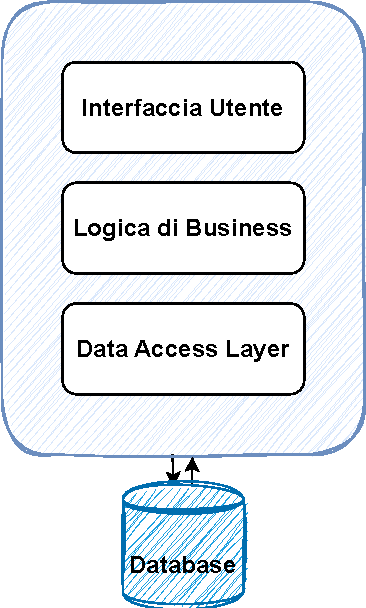
\includegraphics[scale = 0.65]{capitoli/immagini/01_architettura_monolitica.pdf}
    \caption{Architettura Monolitica}
    \label{fig:architettura_monolitica}
\end{figure}

Tale approccio nell'epoca moderna è diventato obsoleto, non è più possibile rilasciare pochi aggiornamenti annuali, che spesso risultano essere solo lavori di manutenzione, con la crescente competizione nel settore, non sviluppare ed integrare nuove funzionalità tende a far perdere interesse verso l'applicativo. L'idea di avere un'applicazione coesa in alcuni casi impone delle limitazioni non indifferenti, per esempio se il servizio di registrazione di un e-commerce non è disponibile per qualche motivo, il resto dell'applicativo deve continuare a funzione, gli utente devono poter cercare prodotti da acquistare e se già registrati, anche di poterli acquistare.

Alcuni degli approcci moderni allo sviluppo di applicazioni sono i seguenti:
\begin{enumerate}
    \item Architettura su più livelli;
    \item Architettura guidata dagli eventi;
    \item Architettura basata sui Microservizi;
\end{enumerate}

\subsection{Architettura su più livelli}
L'architettura su più livelli ha una struttura tradizionale che permette di dividere l'applicazione in diversi livelli che comunicano tra di loro. Un esempio in letteratura è il pattern \ac{MVC}, basato su tre livelli ed utilizzato spesso per lo sviluppo di applicazioni per il web. 

\begin{figure}[h]
    \centering
    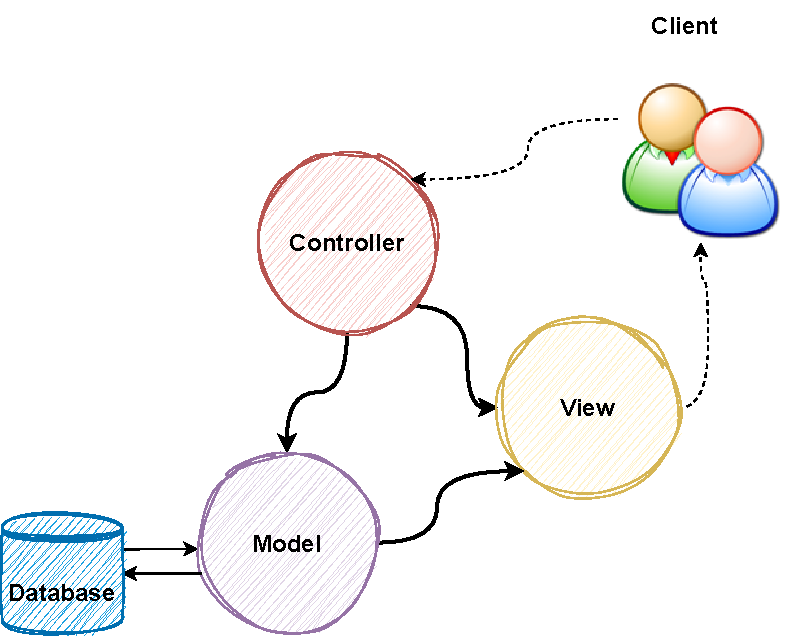
\includegraphics[scale = 0.65]{capitoli/immagini/02_pattern_mvc.pdf}
    \caption{Pattern Model-View-Controll}
    \label{fig:pattern_mvc}
\end{figure}

La suddivisione in livelli permette di semplificare la gestione delle dipendenze e l'esecuzione di funzioni logiche.

\subsection{Architettura guidata dagli eventi}
L'architettura guidata dagli eventi \cite{Event_Drive} è uno stile architetturale dove l'acquisizione, la comunicazione, l'elaborazione e la persistenza degli eventi costituiscono i pilastri portanti della soluzione.

Il fulcro di tale architettura sono gli eventi, per evento si intende qualsiasi avvenimento che porta ad un cambiamento di stato del software o dell'hardware.

L'adozione di tale architettura per la propria applicazione permette di creare un sistema più flessibile che può trasformarsi in base agli eventi, anche in tempo reale. Questo tipo di architettura è il cuore pulsante delle applicazioni sviluppate per l'\ac{IOT} che basa le proprie operazioni sull'acquisizione di dati del mondo reale, come per esempio la temperatura di una stanza o dell'umidità nell'aria, il cambiamento di un parametro che viene monitorato, porta il sistema a reagire di conseguenza.

\begin{figure}[h]
    \centering
    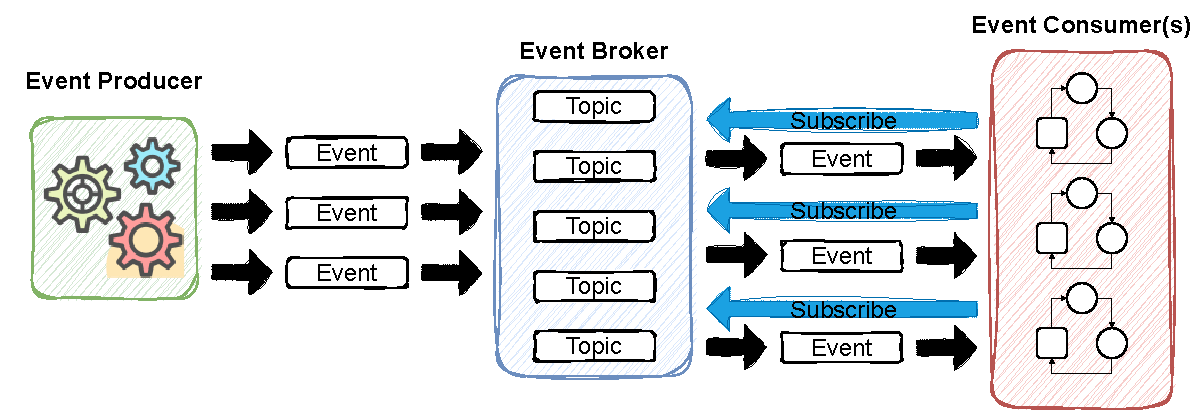
\includegraphics[scale = 0.65]{capitoli/immagini/03_architettura_guidata_dagli_eventi.pdf}
    \caption{Architettura guidata dagli eventi}
    \label{fig:architettura_event_driven}
\end{figure}

\subsection{Architettura basata sui Microservizi}
L'architettura a microservizi descrive un approccio allo sviluppo di software. Tale modello permette di scomporre le applicazioni in diversi componenti, chiamati appunto microservizi, che risultano essere indipendenti l'uno dall'altro. Ogni componente del sistema si occuperà di servire una singola funzionalità.

\begin{figure}[h]
    \centering
    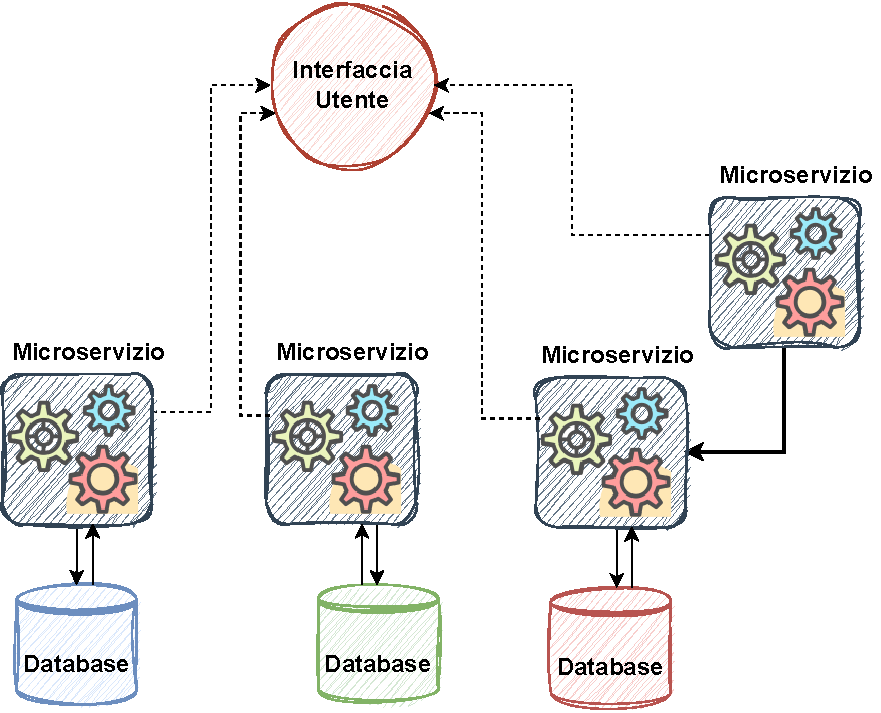
\includegraphics[scale = 0.65]{capitoli/immagini/04_architettura_microservizi.pdf}
    \caption{Architettura a microservizi}
    \label{fig:architettura_microservizi}
\end{figure}

Creando un sistema che si basa sull'approccio ai microservizi, rende la fase di manutenzione dell'applicativo più semplice, permettendo di aggiornare servizi già presenti o di sviluppare e rilasciare nuove funzionalità in un breve lasso di tempo rispetto, per esempio, all'approccio monolitico, che ricordiamo prevede pochi aggiornamenti annuali. Quello di cui abbiamo appena discusso non è l'unico vantaggio, la scalabilità dell'applicazione diventa dinamica, permettendo di gestire in autonomia il carico di lavoro. Il problema del singolo punto di vulnerabilità (Single Point of Failure) viene risolto dalla indipendenza dei microservizi, quando un componente non è disponibile per manutenzione, anomalie o altro, il sistema continuerà ad essere raggiungibile ed utilizzabile dagli utenti.



\begin{comment}
\section{Cloud Computing e Pay As You Go}
Come conseguenza dell'evoluzione della metodologia di sviluppo, ma soprattutto di come è cambiato l'approccio dei clienti, il cloud computing è diventato sempre più presente nella vita di tutti i giorni. La fisiologia alla base del cloud computing si basa sul \ac{PAYG}, non si paga più il software per ricevere una licenza full time oppure un abbonamento come nel caso dei software professionali sviluppati da Adobe (per esempio Adobe Photoshop), ma si paga solo quando il servizio è utilizzato. Un'analogia molto utilizzata per spiegare come funziona questo approccio è pensare alle utenze casalinghe, la corrente elettrica e il gas cittadino venogno pagati in base all'uso in un periodo, se, giustamente, si usa una delle due utenze o entrambe poco, si pagherà di meno rispetto a chi nello stesso periodo ha consumato molto di più.
\end{comment}


\section{Obiettivi}
L'obiettivo di questo lavoro di tesi è quello di esplorare diverse tecnologie che negli ultimi anni si stanno diffondendo, per sviluppare una semplicissima applicazione basata sull'architettura a microservizi, una sorta di Hello World che rappresenta i canoni del modello.

\section{Struttura della Tesi}
La tesi è divisa in quattro capitoli, quello appena concluso ha permesso al lettore di avere una panoramica sull'evoluzione delle architetture utilizzate nello sviluppo di software e del perché è stato necessario allontanarsi dal classico approccio monolitico. Nel prossimo capitolo andremmo ad analizzare e ad esplorare alcuni concetti teorici su cui le tecnologie utilizzate nello sviluppo odierno si basano. Il capitolo tre presenterà le tecnologie che sono state utilizzate per la creazione del software e infine, nel capitolo quattro ci concentreremo sul software sviluppato e sui punti di forza.

Il codice sorgente dell'applicazione è disponibile al seguente link: \url{https://github.com/laurus96/Microservices-Example}